% GNUPLOT: LaTeX picture with Postscript
\begingroup
  \makeatletter
  \providecommand\color[2][]{%
    \GenericError{(gnuplot) \space\space\space\@spaces}{%
      Package color not loaded in conjunction with
      terminal option `colourtext'%
    }{See the gnuplot documentation for explanation.%
    }{Either use 'blacktext' in gnuplot or load the package
      color.sty in LaTeX.}%
    \renewcommand\color[2][]{}%
  }%
  \providecommand\includegraphics[2][]{%
    \GenericError{(gnuplot) \space\space\space\@spaces}{%
      Package graphicx or graphics not loaded%
    }{See the gnuplot documentation for explanation.%
    }{The gnuplot epslatex terminal needs graphicx.sty or graphics.sty.}%
    \renewcommand\includegraphics[2][]{}%
  }%
  \providecommand\rotatebox[2]{#2}%
  \@ifundefined{ifGPcolor}{%
    \newif\ifGPcolor
    \GPcolortrue
  }{}%
  \@ifundefined{ifGPblacktext}{%
    \newif\ifGPblacktext
    \GPblacktexttrue
  }{}%
  % define a \g@addto@macro without @ in the name:
  \let\gplgaddtomacro\g@addto@macro
  % define empty templates for all commands taking text:
  \gdef\gplbacktext{}%
  \gdef\gplfronttext{}%
  \makeatother
  \ifGPblacktext
    % no textcolor at all
    \def\colorrgb#1{}%
    \def\colorgray#1{}%
  \else
    % gray or color?
    \ifGPcolor
      \def\colorrgb#1{\color[rgb]{#1}}%
      \def\colorgray#1{\color[gray]{#1}}%
      \expandafter\def\csname LTw\endcsname{\color{white}}%
      \expandafter\def\csname LTb\endcsname{\color{black}}%
      \expandafter\def\csname LTa\endcsname{\color{black}}%
      \expandafter\def\csname LT0\endcsname{\color[rgb]{1,0,0}}%
      \expandafter\def\csname LT1\endcsname{\color[rgb]{0,1,0}}%
      \expandafter\def\csname LT2\endcsname{\color[rgb]{0,0,1}}%
      \expandafter\def\csname LT3\endcsname{\color[rgb]{1,0,1}}%
      \expandafter\def\csname LT4\endcsname{\color[rgb]{0,1,1}}%
      \expandafter\def\csname LT5\endcsname{\color[rgb]{1,1,0}}%
      \expandafter\def\csname LT6\endcsname{\color[rgb]{0,0,0}}%
      \expandafter\def\csname LT7\endcsname{\color[rgb]{1,0.3,0}}%
      \expandafter\def\csname LT8\endcsname{\color[rgb]{0.5,0.5,0.5}}%
    \else
      % gray
      \def\colorrgb#1{\color{black}}%
      \def\colorgray#1{\color[gray]{#1}}%
      \expandafter\def\csname LTw\endcsname{\color{white}}%
      \expandafter\def\csname LTb\endcsname{\color{black}}%
      \expandafter\def\csname LTa\endcsname{\color{black}}%
      \expandafter\def\csname LT0\endcsname{\color{black}}%
      \expandafter\def\csname LT1\endcsname{\color{black}}%
      \expandafter\def\csname LT2\endcsname{\color{black}}%
      \expandafter\def\csname LT3\endcsname{\color{black}}%
      \expandafter\def\csname LT4\endcsname{\color{black}}%
      \expandafter\def\csname LT5\endcsname{\color{black}}%
      \expandafter\def\csname LT6\endcsname{\color{black}}%
      \expandafter\def\csname LT7\endcsname{\color{black}}%
      \expandafter\def\csname LT8\endcsname{\color{black}}%
    \fi
  \fi
  \setlength{\unitlength}{0.0500bp}%
  \begin{picture}(7200.00,5040.00)%
    \gplgaddtomacro\gplbacktext{%
      \csname LTb\endcsname%
      \put(1210,704){\makebox(0,0)[r]{\strut{} 0}}%
      \put(1210,1395){\makebox(0,0)[r]{\strut{} 20}}%
      \put(1210,2086){\makebox(0,0)[r]{\strut{} 40}}%
      \put(1210,2778){\makebox(0,0)[r]{\strut{} 60}}%
      \put(1210,3469){\makebox(0,0)[r]{\strut{} 80}}%
      \put(1210,4160){\makebox(0,0)[r]{\strut{} 100}}%
      \put(1342,484){\makebox(0,0){\strut{} 0}}%
      \put(2033,484){\makebox(0,0){\strut{} 5}}%
      \put(2724,484){\makebox(0,0){\strut{} 10}}%
      \put(3415,484){\makebox(0,0){\strut{} 15}}%
      \put(4106,484){\makebox(0,0){\strut{} 20}}%
      \put(4797,484){\makebox(0,0){\strut{} 25}}%
      \put(5488,484){\makebox(0,0){\strut{} 30}}%
      \put(6179,484){\makebox(0,0){\strut{} 35}}%
      \put(6870,484){\makebox(0,0){\strut{} 40}}%
      \put(700,2432){\rotatebox{90}{\makebox(0,0){\strut{}True Positive Rate}}}%
      \put(4106,154){\makebox(0,0){\strut{}False Positive Rate}}%
      \put(4106,4710){\makebox(0,0){\strut{}R.O.C.}}%
      \put(4106,4490){\makebox(0,0){\strut{} Parameter: VFH Threshold}}%
    }%
    \gplgaddtomacro\gplfronttext{%
      \csname LTb\endcsname%
      \put(5883,1977){\makebox(0,0)[r]{\strut{}Furniture Detection (Unfiltered)}}%
      \csname LTb\endcsname%
      \put(5883,1757){\makebox(0,0)[r]{\strut{}Furniture Detection (Filtered)}}%
      \csname LTb\endcsname%
      \put(5883,1537){\makebox(0,0)[r]{\strut{}VFH Full (Unfiltered)}}%
      \csname LTb\endcsname%
      \put(5883,1317){\makebox(0,0)[r]{\strut{}VFH Full (Filtered)}}%
      \csname LTb\endcsname%
      \put(5883,1097){\makebox(0,0)[r]{\strut{}VFH Partial (Unfiltered)}}%
      \csname LTb\endcsname%
      \put(5883,877){\makebox(0,0)[r]{\strut{}VFH Partial (Filtered)}}%
    }%
    \gplbacktext
    \put(0,0){\includegraphics{images/ROC-vfh-vs-fd.eps}}%
    \gplfronttext
  \end{picture}%
\endgroup
